\chapter{Real Numbers} \label{rn:chapter}

%%%%%%%%%%%%%%%%%%%%%%%%%%%%%%%%%%%%%%%%%%%%%%%%%%%%%%%%%%%%%%%%%%%%%%%%%%%%%%

\section{Basic properties} \label{sec:basicpropsrn}

\sectionnotes{1.5 lectures}

The main object we work with in analysis is the set of
\myindex{real numbers}.  As this set is so fundamental, often much time is
spent on formally constructing the set of real numbers.  However, we 
take an easier approach here and just assume that a set with the correct
properties exists.  We start with the definitions of those
properties.

\begin{defn}
An \emph{\myindex{ordered set}} is a set $S$ together with
a relation $<$ such that
%\begin{enumerate}[(i),itemsep=0.5\itemsep,parsep=0.5\parsep,topsep=0.5\topsep,partopsep=0.5\partopsep]
%\begin{enumerate}[(i),nolistsep]
\begin{enumerate}[(i)]
\item \emph{(\myindex{trichotomy})} For all $x, y \in S$, exactly one of
$x < y$, $x=y$, or $y < x$ holds.
\item \emph{(transitivity)} If $x,y,z \in S$ are such that $x < y$ and $y
< z$, then $x < z$.
\end{enumerate}
We write $x \leq y$ if $x < y$ or $x=y$.  We define
$>$ and $\geq$ in the obvious way.
\glsadd{not:ordereq}
\glsadd{not:orderlt}
\glsadd{not:orderleq}
\glsadd{not:ordergt}
\glsadd{not:ordergeq}
\end{defn}


The set of rational numbers $\Q$ is an ordered set by letting
$x < y$ if and only if $y-x$ is a positive rational number, that is
if $y-x = \nicefrac{p}{q}$ where $p,q \in \N$.  Similarly,
$\N$ and $\Z$ are also ordered sets.

There are other ordered sets than sets of numbers.  For example, the
set of countries can be ordered by landmass, so India $>$
Lichtenstein.
A typical ordered set that you have used since primary school is the
dictionary.  It is the ordered set of words where the order is the
so-called lexicographic ordering.  Such ordered sets often appear, for
example, in
computer science.  In this book we will mostly be interested in ordered
sets of numbers.

\begin{defn}
Let $E \subset S$, where $S$ is an ordered set.
%\begin{enumerate}[(i),itemsep=0.5\itemsep,parsep=0.5\parsep,topsep=0.5\topsep,partopsep=0.5\partopsep]
%\begin{enumerate}[(i),nolistsep]
\begin{enumerate}[(i)]
\item If there exists a $b \in S$ such that $x \leq b$ for all $x \in E$,
then we say $E$ is \emph{\myindex{bounded above}} and $b$
is an \emph{\myindex{upper bound}} of $E$.
\item If there exists a $b \in S$ such that $x \geq b$ for all $x \in E$,
then we say $E$ is \emph{\myindex{bounded below}} and $b$
is a \emph{\myindex{lower bound}} of $E$.
\item If there exists an upper bound $b_0$ of $E$ such that whenever
$b$ is an upper bound for $E$ we have $b_0 \leq b$, then $b_0$
is called the \emph{\myindex{least upper bound}} or
the \emph{\myindex{supremum}}
of $E$.  See \figureref{fig:lub}.  We write\glsadd{not:sup}
\begin{equation*}
\sup\, E := b_0  .
\end{equation*}
\item Similarly, if there exists a lower bound $b_0$ of $E$ such that whenever
$b$ is a lower bound for $E$ we have $b_0 \geq b$, then $b_0$
is called the \emph{\myindex{greatest lower bound}} or
the \emph{\myindex{infimum}}
of $E$.  We write\glsadd{not:inf}
\begin{equation*}
\inf\, E := b_0  .
\end{equation*}
\end{enumerate}
When a set $E$ is both bounded above and bounded below, we say simply that
$E$ is \emph{bounded}\index{bounded set}.
\end{defn}

The notation $\sup E$ and $\inf E$ is justified as
the
supremum (or infimum) is unique (if it exists): If $b$ and
$b'$ are suprema of $E$, then $b \leq b'$ and $b' \leq b$, because both
$b$ and $b'$ are the least upper bounds, so $b=b'$.


\begin{myfigureht}
\subimport*{figures/}{lub.pdf_t}
\caption{A set $E$ bounded above and the least upper bound of $E$.\label{fig:lub}}
\end{myfigureht}

A simple example:
Let $S := \{ a, b, c, d, e \}$ be ordered as $a < b < c < d < e$, and
let $E := \{ a, c \}$.  Then $c$, $d$, and $e$ are upper bounds of $E$, and
$c$ is the least upper bound or supremum of $E$.

A supremum or infimum for $E$ (even if it exists) need not be
in $E$.  The set $E := \{ x \in \Q : x < 1 \}$ has a least upper
bound of 1, but 1 is not in the set $E$ itself.
The set 
$G := \{ x \in \Q : x \leq 1 \}$ also has an upper bound of 1,
and in this case $1 \in G$.  
The set $P := \{ x \in \Q : x \geq 0 \}$ has no upper bound (why?) and therefore
it cannot have a least upper bound.  The set $P$ does have a greatest lower
bound:~0.

\begin{defn} \label{defn:lub}
An ordered set $S$ has the \emph{\myindex{least-upper-bound property}} if
every nonempty
subset $E \subset S$ that is bounded above has a least upper bound,
that is $\sup\, E$ exists in $S$.
\end{defn}

The \emph{least-upper-bound property}
is sometimes called the \emph{\myindex{completeness property}} or the
\emph{\myindex{Dedekind completeness property}}%
\footnote{%
Named after the German mathematician
\href{https://en.wikipedia.org/wiki/Richard_Dedekind}{Julius Wilhelm Richard Dedekind}
(1831--1916).}.
As we will note in the
next section, the real numbers have this property.

\begin{example}
The set $\Q$ of rational numbers does not have the least-upper-bound property.  The subset
$\{ x \in \Q : x^2 < 2 \}$ does not have a supremum in $\Q$.  We will
see later (\exampleref{example:sqrt2}) that the supremum is 
$\sqrt{2}$, which is not rational%
\footnote{This is true for all other roots of 2, and interestingly,
the fact that $\sqrt[k]{2}$ is never rational for $k > 1$ implies no piano can
ever be perfectly tuned in all keys.  See for example:
\url{https://youtu.be/1Hqm0dYKUx4}.}.
Suppose $x \in \Q$ such that $x^2 = 2$.
Write $x=\nicefrac{m}{n}$ in lowest terms.  So ${(\nicefrac{m}{n})}^2 = 2$
or
$m^2 = 2n^2$.  Hence, $m^2$ is divisible by 2, and so $m$ is divisible by
2.  Write $m = 2k$ and so ${(2k)}^2 = 2n^2$.  Divide by 2
and note that $2k^2 = n^2$, and hence $n$ is divisible by 2.  But that is a
contradiction as $\nicefrac{m}{n}$ is in lowest terms.
\end{example}

That $\Q$ does not have the least-upper-bound property is one of the most
important reasons why we work with $\R$ in analysis.  The set $\Q$
is just fine for algebraists.  But us analysts require the least-upper-bound
property to do any work.
We also require our real numbers to have many algebraic properties.  In
particular, we require that they are a field.


%\enlargethispage{\baselineskip}
\begin{defn}
A set $F$ is called a \emph{\myindex{field}} if it has two operations
defined on it, addition $x+y$ and multiplication $xy$, and if it satisfies
the following axioms\index{axiom}:
%mbxSTARTIGNORE
\begin{enumerate}[({A}1)]
%mbxENDIGNORE
%mbxCLOSEPARAGRAPH
%mbx <dl>
\item
%mbx <title>(A1)</title>
If $x \in F$ and $y \in F$, then $x+y \in F$.
\item
%mbx <title>(A2)</title>
\emph{(commutativity of addition)}
$x+y = y+x$ for all $x,y \in F$.
\item
%mbx <title>(A3)</title>
\emph{(associativity of addition)}
$(x+y)+z = x+(y+z)$ for all $x,y,z \in F$.
\item
%mbx <title>(A4)</title>
There exists an element $0 \in F$ such that
$0+x = x$ for all $x \in F$.
\item
%mbx <title>(A5)</title>
For every element $x\in F$, there exists an element $-x \in F$
such that $x + (-x) = 0$.
%mbxCLOSEITEM
%mbx </dl>
%mbxSTARTIGNORE
\end{enumerate}
\begin{enumerate}[({M}1)]
%mbxENDIGNORE
%mbx <dl>
\item
%mbx <title>(M1)</title>
If $x \in F$ and $y \in F$, then $xy \in F$.
\item
%mbx <title>(M2)</title>
\emph{(commutativity of multiplication)}
$xy = yx$ for all $x,y \in F$.
\item
%mbx <title>(M3)</title>
\emph{(associativity of multiplication)}
$(xy)z = x(yz)$ for all $x,y,z \in F$.
\item
%mbx <title>(M4)</title>
There exists an element $1 \in F$ (and $1 \not= 0$) such that
$1x = x$ for all $x \in F$.
\item
%mbx <title>(M5)</title>
For every $x\in F$ such that $x \not= 0$ there exists an element
$\nicefrac{1}{x} \in F$
such that $x(\nicefrac{1}{x}) = 1$.
%\end{enumerate}
%\begin{enumerate}
%mbxSTARTIGNORE
\item[(D)]
%mbxENDIGNORE
%mbxlatex \item
%mbx <title>(D)</title>
\emph{(distributive law)} $x(y+z) = xy+xz$
for all $x,y,z \in F$.
%mbxSTARTIGNORE
\end{enumerate}
%mbxENDIGNORE
%mbxCLOSEITEM
%mbx </dl>
\end{defn}

\begin{example}
The set $\Q$ of rational numbers is a field.  On the other hand $\Z$ is not a
field, as it does not contain multiplicative inverses.  For example,
there is no $x \in \Z$ such that $2x = 1$, so (M5) is not satisfied.  You
can check that (M5) is the only property that fails\footnote{An algebraist would say that $\Z$ is an ordered
ring, or perhaps more precisely a commutative ordered ring.}.
\end{example}

We will assume the basic facts about fields that are easily 
proved from the axioms.  For example, $0x = 0$ is easily proved
by noting that $xx = (0+x)x = 0x+xx$, using (A4), (D)\@, and (M2).  Then
using (A5) on $xx$, along with (A2), (A3), and (A4), we obtain $0 = 0x$.

\begin{defn}
A field $F$ is said to be an \emph{\myindex{ordered field}} if
$F$ is also an ordered set such that
\begin{enumerate}[(i)]
\item \label{defn:ordfield:i} For $x,y,z \in F$,  $x < y$ implies $x+z <
y+z$.
\item \label{defn:ordfield:ii} For $x,y \in F$, $x > 0$ and $y > 0$
implies $xy > 0$.
\end{enumerate}
If $x > 0$, we say $x$ is \emph{\myindex{positive}}.
If $x < 0$, we say $x$ is \emph{\myindex{negative}}.
We also say $x$ is \emph{\myindex{nonnegative}} if $x \geq 0$,
and $x$ is \emph{\myindex{nonpositive}} if $x \leq 0$.
\end{defn}

It can be checked that the rational numbers $\Q$ with the
standard ordering is an ordered field.

\begin{prop} \label{prop:bordfield}
Let $F$ be an ordered field and $x,y,z,w \in F$.  Then
\begin{enumerate}[(i)]
\item \label{prop:bordfield:i} If $x > 0$, then $-x < 0$ (and vice versa).
\item \label{prop:bordfield:ii} If $x > 0$ and $y < z$, then $xy < xz$.
\item \label{prop:bordfield:iii} If $x < 0$ and $y < z$, then $xy > xz$.
\item \label{prop:bordfield:iv} If $x \not= 0$, then $x^2 > 0$.
\item \label{prop:bordfield:v} If $0 < x < y$, then $0 < \nicefrac{1}{y} < \nicefrac{1}{x}$.
\item \label{prop:bordfield:vi} If $0 < x < y$, then $x^2 < y^2$.
\item \label{prop:bordfield:vii} If $x \leq y$ and $z \leq w$, then $x + z \leq y + w$.
\end{enumerate}
\end{prop}

Note that \ref{prop:bordfield:iv} implies in particular that $1 > 0$.

\begin{proof}
Let us prove \ref{prop:bordfield:i}.  The inequality $x > 0$ implies by item
\ref{defn:ordfield:i} of definition of ordered fields that
$x + (-x) > 0 + (-x)$.  Apply the algebraic properties of fields to
obtain $0 > -x$.  The \myquote{vice versa} follows by similar calculation.

For \ref{prop:bordfield:ii}, notice that $y < z$ implies
$0 < z - y$ by
item \ref{defn:ordfield:i} of the definition of ordered fields.  
Apply item 
\ref{defn:ordfield:ii} of the definition of ordered fields to obtain
$0 < x(z-y)$.  By algebraic properties, $0 < xz - xy$.
Again by item
\ref{defn:ordfield:i} of the definition, $xy < xz$.

Part \ref{prop:bordfield:iii} is left as an exercise.

To prove part \ref{prop:bordfield:iv}, first suppose $x > 0$.
By item 
\ref{defn:ordfield:ii} of the definition of ordered fields,
$x^2 > 0$ (use $y=x$).  If $x < 0$, we use 
part \ref{prop:bordfield:iii} of this proposition, where we plug in $y=x$ and
$z=0$.

To prove part \ref{prop:bordfield:v}, notice that
$\nicefrac{1}{x}$ cannot be equal to zero (why?).
Suppose $\nicefrac{1}{x} < 0$,
then $\nicefrac{-1}{x} > 0$ by \ref{prop:bordfield:i}.
Apply part \ref{defn:ordfield:ii} of the definition (as $x > 0$) to obtain
$x(\nicefrac{-1}{x}) > 0$ or $-1 > 0$, which contradicts $1 > 0$ by using part
\ref{prop:bordfield:i} again.  Hence $\nicefrac{1}{x} > 0$.
Similarly, $\nicefrac{1}{y} > 0$.  Thus $(\nicefrac{1}{x})(\nicefrac{1}{y}) > 0$
by definition of ordered field, and by part \ref{prop:bordfield:ii},
\begin{equation*}
(\nicefrac{1}{x})(\nicefrac{1}{y})x < (\nicefrac{1}{x})(\nicefrac{1}{y})y .
\end{equation*}
By algebraic properties, $\nicefrac{1}{y} < \nicefrac{1}{x}$.

Parts \ref{prop:bordfield:vi} and \ref{prop:bordfield:vii} are left as
exercises.
\end{proof}

The product of two positive numbers (elements of an ordered field) is positive.
However, it is not true that if the product is positive, then each of the two
factors must be positive.  For instance, $(-1)(-1) = 1 > 0$.

\begin{prop}
Let $x,y \in F$, where $F$ is an ordered field.  If
$xy > 0$, then either both $x$ and $y$ are positive, or both are negative.
\end{prop}

\begin{proof}
We show the contrapositive: If either one of $x$ or $y$ is zero, or
if $x$ and $y$ have opposite signs, then $xy$ is not positive.
If either
$x$ or $y$ is zero, then $xy$ is zero and hence not positive.
Hence assume that $x$ and $y$ are nonzero and have
opposite signs.
Without loss of
generality suppose $x > 0$ and $y < 0$.  Multiply $y < 0$ by $x$ to get
$xy < 0x = 0$.
\end{proof}

\begin{example} \label{example:complexfield}
The reader may also know about the \emph{\myindex{complex numbers}},
usually denoted by
$\C$.\glsadd{not:complex}  That is, $\C$ is the set of numbers of
the form $x + iy$, where $x$ and $y$ are real numbers, and $i$ is the
imaginary number, a number such that $i^2 = -1$.  The reader may
remember from algebra that $\C$ is also a field; however, it is not an
ordered field.  While one can make $\C$ into an ordered set in some way,
it is not possible to put an
order on $\C$ that would make it an ordered field: In every ordered field,
$-1 < 0$ and $x^2 > 0$ for all nonzero $x$, but in $\C$, $i^2 = -1$.
\end{example}

Finally, an ordered field that has the least-upper-bound property has the
corresponding property for greatest lower bounds.

\begin{prop}
Let $F$ be an ordered field with the least-upper-bound property.
Let $A \subset F$ be a nonempty set that is bounded below.
Then $\inf\, A$ exists.
\end{prop}

\begin{proof}
Let $B := \{ -x : x \in A \}$. Let $b \in F$ be a lower bound for $A$:
If $x \in A$, then $x \geq b$. In other words, $-x \leq -b$.  So $-b$
is an upper bound for $B$.
Since $F$ has the least-upper-bound property, $c:=\sup\, B$ exists, and $c \leq -b$.
As $y \leq c$
for all $y \in B$, then $-c \leq x$ for all $x \in A$.
So
$-c$ is a lower bound for $A$.  As $-c \geq b$,
$-c$ is the greatest lower bound of $A$.
\end{proof}

\subsection{Exercises}

\begin{exercise}
Prove part \ref{prop:bordfield:iii} of \propref{prop:bordfield}.
That is, let $F$ be an ordered field and $x,y,z \in F$.  Prove
If $x < 0$ and $y < z$, then $xy > xz$.
\end{exercise}


\begin{exercise} \label{exercise:finitesethasminmax}
Let $S$ be an ordered set.  Let $A \subset S$ be a nonempty finite subset.
Then $A$ is bounded.  Furthermore,
$\inf\, A$ exists and is in $A$ and 
$\sup\, A$ exists and is in $A$.  Hint: Use
\hyperref[induction:thm]{induction}.
\end{exercise}

\begin{exercise} \label{exercise:squareineq}
Prove part \ref{prop:bordfield:vi} of \propref{prop:bordfield}.
That is, let $x, y \in F$, where $F$ is an ordered field, such that
$0 < x < y$.  Show that $x^2 < y^2$.
\end{exercise}

\begin{exercise}
Let $S$ be an ordered set.  Let $B \subset S$ be bounded (above and
below).  Let $A \subset B$ be a nonempty subset.
Suppose all the $\inf$s and
$\sup$s exist. Show that
\begin{equation*}
\inf\, B \leq \inf\, A \leq \sup\, A \leq \sup\, B .
\end{equation*}
\end{exercise}

\begin{exercise}
Let $S$ be an ordered set.  Let $A \subset S$ and suppose 
$b$ is an upper bound for $A$.  Suppose $b \in A$.  Show
that $b = \sup\, A$.
\end{exercise}

\begin{exercise}
Let $S$ be an ordered set.  Let $A \subset S$ be nonempty and
bounded above.
Suppose $\sup\, A$ exists and
$\sup\, A \notin A$.
Show that $A$ contains a countably infinite
subset.
%In particular, $A$ is infinite.
\end{exercise}

\begin{exercise}
Find a (nonstandard) ordering of the set of natural numbers $\N$
such that there exists a nonempty proper subset $A \subsetneq \N$
and such that $\sup\, A$ exists in $\N$, but $\sup\, A \notin A$.
To keep things straight it might be a good idea to use a different
notation for the nonstandard ordering such as $n \prec m$.
\end{exercise}

\begin{exercise}
Let $F := \{ 0, 1, 2 \}$.
\begin{enumerate}[a)]
\item
Prove that there is
exactly one way to define addition and multiplication so that $F$ is
a field if $0$ and $1$ have their usual meaning of (A4) and (M4).
\item
Show that $F$ cannot be an ordered field.
\end{enumerate}
\end{exercise}

\begin{exercise} \label{exercise:dominatingb}
Let $S$ be an ordered set and
$A$ is a nonempty subset such that $\sup \, A$ exists.  Suppose there
is a $B \subset A$ such that whenever $x \in A$ there is a $y \in B$
such that $x \leq y$.  Show that $\sup \, B$ exists and $\sup \, B = \sup \, A$.
\end{exercise}

\begin{exercise}
Let $D$ be the ordered set of all possible words (not just English words,
all strings of letters of arbitrary length)
using the Latin alphabet using only lower case letters.  The order is the
lexicographic order as in a dictionary (e.g.\ \emph{aa} $<$ \emph{aaa} $<$ \emph{dog} $<$ \emph{door}).
Let $A$ be the subset of $D$ containing the words whose
first letter is `a' (e.g.\ \emph{a} $\in A$, \emph{abcd} $\in A$).
Show that $A$ has a supremum and find what it is.
\end{exercise}

\begin{exercise}
Let $F$ be an ordered field and $x,y,z,w \in F$.
\begin{enumerate}[a)]
\item
Prove part \ref{prop:bordfield:vii} of \propref{prop:bordfield}.
That is,
if $x \leq y$ and $z \leq w$, then $x+z \leq y+w$.
\item
Prove that
if $x < y$ and $z \leq w$, then $x+z < y+w$.
\end{enumerate}
\end{exercise}

\begin{exercise}
Prove that any ordered field must contain a countably infinite set.
\end{exercise}

\begin{exercise}
Let $\N_{\infty} := \N \cup \{ \infty \}$, where elements of $\N$ are
ordered in the usual way amongst themselves,
and $k < \infty$ for every $k \in \N$.  Show $\N_{\infty}$ is an ordered set
and that every subset $E \subset \N_{\infty}$ has a supremum in
$\N_{\infty}$ (make sure to also handle the case of an empty set).
\end{exercise}

\begin{exercise}
Let $S := \{ a_k : k \in \N \} \cup \{ b_k : k \in \N \}$, ordered such that
$a_k < b_j$ for every $k$ and $j$,
$a_k < a_m$ whenever $k < m$,
and $b_k > b_m$ whenever $k < m$.
\begin{enumerate}[a)]
\item
Show that $S$ is an ordered set.
\item
Show that every subset of $S$ is bounded (both above and below).
\item
Find a bounded subset of $S$ that has no least upper bound.
\end{enumerate}
\end{exercise}

%%%%%%%%%%%%%%%%%%%%%%%%%%%%%%%%%%%%%%%%%%%%%%%%%%%%%%%%%%%%%%%%%%%%%%%%%%%%%%

\sectionnewpage
\section{The set of real numbers} \label{sec:setofreals}

\sectionnotes{2 lectures, the extended real numbers are optional}

\subsection{The set of real numbers}

We finally get to the real number system.  To simplify matters, instead of constructing the
real number set from the rational numbers, we simply state their existence
as a theorem without proof.  Notice that $\Q$ is an ordered
field.

\begin{thm}
There exists a unique\footnote{Uniqueness is up to isomorphism, but we wish
to avoid excessive use of algebra.  For us, it is simply enough to assume
that a set of real numbers exists.  See Rudin~\cite{Rudin:baby} for the
construction and more details.}
ordered field $\R$ with the \hyperref[defn:lub]{least-upper-bound property}
such that $\Q \subset \R$.
\end{thm}

Note that also $\N \subset \Q$.  We saw that $1 > 0$.  By
\hyperref[induction:thm]{induction}
(exercise) we can prove that
$n > 0$ for all $n \in \N$.
Similarly, we verify simple statements about rational numbers.
For example, we proved that if $n > 0$, then $\nicefrac{1}{n} > 0$.
Then $m < k$ implies $\nicefrac{m}{n} < \nicefrac{k}{n}$.

Analysis consists of proving inequalities, and
the following proposition, or one of its many variations,
is how an analyst proves a nonstrict inequality.

\begin{prop}
If $x \in \R$ is such that $x \leq \epsilon$ for all
$\epsilon \in \R$ where
$\epsilon > 0$, then $x \leq 0$.
\end{prop}

\begin{proof}
If $x > 0$, then $0 < \nicefrac{x}{2} < x$ (why?).  Taking
$\epsilon = \nicefrac{x}{2}$ obtains a contradiction.  Thus $x \leq 0$.
\end{proof}

For nonnegative $x$, an equality results:
\emph{If $x \geq 0$ is such that $x \leq \epsilon$ for all
$\epsilon > 0$, then $x = 0$.}
A common version uses the absolute value (see \sectionref{sec:absval}):
\emph{If $\sabs{x} \leq \epsilon$ for all
$\epsilon > 0$, then $x = 0$.}
To prove $x \geq 0$, an analyst might prove
that $x \geq -\epsilon$ for all $\epsilon > 0$.
From now on, when we say $x \geq 0$ or
$\epsilon > 0$, we automatically mean that $x \in \R$ and $\epsilon \in \R$.

The idea behind the proposition above is that
any time we have two real numbers $a < b$, then there is another
real number $c$ such that
$a < c < b$.  Infinitely many such $c$ exist.  One of them is, for example,
$c = \frac{a+b}{2}$ (why?).
We will use this fact in the next example.

The most useful property of $\R$ for analysts
is not just that it is an ordered field, but that it has the
\hyperref[defn:lub]{least-upper-bound property}.  Essentially, we want $\Q$, but we also
want to take suprema (and infima) willy-nilly.  So what we do is 
take $\Q$ and
throw in enough numbers to obtain $\R$.

We mentioned already that $\R$ contains elements that are not in $\Q$
because of the \hyperref[defn:lub]{least-upper-bound property}.  Let us
prove it.
We saw there is no
rational square root of two.  The set
$\{ x \in \Q : x^2 < 2 \}$ implies the existence of the real number
$\sqrt{2}$, although this fact requires a bit of work.  See also
\exerciseref{exercise:sqrt2QorR}.

\begin{example} \label{example:sqrt2}
Claim: \emph{There exists a unique positive
$r \in \R$ such that $r^2 = 2$.  We denote $r$ by $\sqrt{2}$.}

\begin{proof}
Take the set
$A := \{ x \in \R : x^2 < 2 \}$.  We first show that $A$ is bounded above and
nonempty.  The equation $x \geq 2$ implies $x^2 \geq 4$
(see \exerciseref{exercise:squareineq}), so
if $x^2 < 2$, then $x < 2$, and $A$ is bounded above.
As $1 \in A$, the set $A$ is nonempty.  We can therefore find the supremum.

Let $r := \sup\, A$.  We will show that $r^2 = 2$ by showing
that $r^2 \geq 2$ and $r^2 \leq 2$.  This is the way analysts show
equality, by showing two inequalities.
We already know that $r \geq 1 > 0$.

%\medskip
In the following, it may seem we are pulling certain expressions out of
a hat.  When writing a proof such as this we would, of course, come up with
the expressions only after playing around with what we wish to prove.  The
order in which we write the proof is not necessarily the order in which we
come up with the proof.

Let us first show that $r^2 \geq 2$.
Take a positive number $s$ such that $s^2 < 2$.  We wish to find an $h > 0$
such that ${(s+h)}^2 < 2$.
As $2-s^2 > 0$, we have $\frac{2-s^2}{2s+1} > 0$.
Choose an $h \in \R$ such that
$0 < h < \frac{2-s^2}{2s+1}$.
Furthermore, assume $h < 1$.  Estimate,
\begin{equation*}
\begin{aligned}
{(s+h)}^2 - s^2 & = h(2s + h) \\
 & < h(2s+1) & & \quad \bigl(\text{since } h < 1\bigr) \\
 & < 2-s^2 & & \quad \bigl(\text{since } h < \tfrac{2-s^2}{2s+1} \bigr) .
\end{aligned}
\end{equation*}
Therefore, ${(s+h)}^2 < 2$.  Hence $s+h \in A$, but as $h > 0$,
we have $s+h > s$.  So $s < r = \sup\, A$.  As $s$ was an arbitrary
positive number such that $s^2 < 2$, it follows that $r^2 \geq 2$.

%\medskip

Now take a positive number $s$ such that
$s^2 > 2$.  We wish to find an $h > 0$ such that
${(s-h)}^2 > 2$ and $s-h$ is still positive.
As 
$s^2-2 > 0$, we have $\frac{s^2-2}{2s} > 0$.
Let $h := \frac{s^2-2}{2s}$,
and check
$s-h=s-\frac{s^2-2}{2s} = \frac{s}{2}+\frac{1}{s} > 0$.  Estimate,
\begin{equation*}
\begin{aligned}
s^2 - {(s-h)}^2 & = 2sh - h^2 \\
 & < 2sh & & \quad \bigl( \text{since } h^2 > 0 \text{ as } h \not= 0 \bigr)  \\
 & = s^2-2 & & \quad \bigl( \text{since } h = \tfrac{s^2-2}{2s} \bigr) .
\end{aligned}
\end{equation*}
By subtracting $s^2$ from both sides and multiplying by $-1$, we find
${(s-h)}^2 > 2$.  Therefore, $s-h \notin A$.

Moreover, if $x \geq s-h$,
then $x^2 \geq {(s-h)}^2 > 2$ (as $x > 0$ and $s-h > 0$) and so $x \notin A$.
Thus,
$s-h$ is an upper bound for $A$.  However, $s-h < s$,  or in other
words, $s > r = \sup\, A$.  Hence, $r^2 \leq 2$.

\medskip

Together, $r^2 \geq 2$ and $r^2 \leq 2$ imply
$r^2 = 2$.  The existence part is finished.  We still need to
handle uniqueness.  Suppose $s \in \R$ such that $s^2 = 2$ and $s > 0$.
Thus $s^2 = r^2$.  However, if $0 < s < r$, then $s^2 < r^2$.  Similarly,
$0 < r < s$ implies $r^2 < s^2$.  Hence $s = r$.
\end{proof}
\end{example}

The number $\sqrt{2} \notin \Q$.  The set
$\R \setminus \Q$ is called the set of
\emph{\myindex{irrational}} numbers.  We just saw that $\R \setminus \Q$
is nonempty.  Not only is it nonempty, we will see later that it is very
large indeed.

Using the same technique as above, we can show that a positive real
number $x^{1/n}$ exists for all $n\in \N$ and all $x > 0$.
That is, for each $x > 0$,
there exists a unique positive real number $r$ such that $r^n = x$.
The proof is left as an exercise.

\subsection{Archimedean property}

As we have seen, there are plenty of real numbers in any interval.  But
there are also infinitely many rational numbers in any interval.  The
following is one of the fundamental facts about the real numbers.
The two parts of the next theorem are actually equivalent, even though it may
not seem like that at first sight.


\begin{thm} \label{thm:arch}
%FIXMEevillayouthack
\pagebreak[3]
\leavevmode
\begin{enumerate}[(i)]
\item \label{thm:arch:i} \emph{(\myindex{Archimedean property})}%
\footnote{Named after the Ancient Greek mathematician
\href{https://en.wikipedia.org/wiki/Archimedes}{Archimedes of Syracuse}
(c.\ 287 BC -- c.\ 212 BC)\@.
This property is Axiom V from Archimedes' \myquote{On the Sphere and
Cylinder} 225
BC\@.}
If $x, y \in \R$ and
$x > 0$, then there exists an $n \in \N$ such that
\begin{equation*}
nx > y .
\end{equation*}
\item \label{thm:arch:ii} \emph{($\Q$ is dense in $\R$\index{density of
rational numbers})} If $x, y \in \R$ and
$x < y$, then there exists an $r \in \Q$ such that
$x < r < y$.
\end{enumerate}
\end{thm}

\begin{proof}
Let us prove \ref{thm:arch:i}.  Divide through by $x$.
Then \ref{thm:arch:i} says that for every real number $t:= \nicefrac{y}{x}$,
we can find $n \in \N$ such that $n > t$.  In other words,
\ref{thm:arch:i} says that $\N \subset \R$ is not bounded above.
Suppose for contradiction that $\N$ is bounded above.  Let $b := \sup \N$.
The number $b-1$ cannot possibly be an upper bound for $\N$ as it is strictly
less than $b$ (the least upper bound).  Thus there exists an $m \in \N$ such that $m > b-1$.
Add one to obtain $m+1 > b$, contradicting $b$ being an
upper bound.

\begin{myfigureht}
\subimport*{figures/}{figdensofQ.pdf_t}
\caption{Idea of the proof of the density of $\Q$: Find $n$ such that $y-x >
\nicefrac{1}{n}$, then take the least $m$ such that $\nicefrac{m}{n} > x$.\label{figdensofQ}}
\end{myfigureht}
Let us tackle \ref{thm:arch:ii}.
See \figureref{figdensofQ}
for a picture of the idea behind the proof.
First assume $x \geq 0$.
Note that $y-x > 0$.
By \ref{thm:arch:i}, there exists an $n \in \N$ such that
\begin{equation*}
n(y-x) > 1
\qquad \text{or} \qquad
y-x > \nicefrac{1}{n}.
\end{equation*}
Again by \ref{thm:arch:i} the set 
$A := \{ k \in \N : k > nx \}$ is nonempty.  By the
\hyperlink{wop:link}{well ordering property}
of $\N$, $A$ has a least element $m$, and as $m \in A$,
then $m > nx$.
Divide through by $n$ to get $x < \nicefrac{m}{n}$.
As $m$ is the least
element of $A$, $m-1 \notin A$.
If $m > 1$, then $m-1 \in \N$, but $m-1 \notin A$ and so $m-1 \leq nx$.
If $m=1$,
then $m-1 = 0$, and $m-1 \leq nx$ still holds as $x \geq 0$.
In other words,
\begin{equation*}
m-1 \leq nx \qquad \text{or} \qquad m \leq nx+1 .
\end{equation*}
On the other hand,
from $n(y-x) > 1$ we obtain $ny > 1+nx$.
Hence $ny > 1+nx \geq m$, and therefore $y > \nicefrac{m}{n}$.
Putting everything together we obtain $x < \nicefrac{m}{n} < y$.
So take $r = \nicefrac{m}{n}$.

Now assume $x < 0$.  If $y > 0$, then just take $r=0$.  If
$y \leq 0$, then $0 \leq -y < -x$, and we
find a rational $q$ such that $-y < q < -x$.  Then take $r = -q$.
\end{proof}

Let us state and prove a simple but useful corollary of the
\hyperref[thm:arch:i]{Archimedean property}.

\begin{cor}
$\inf \{ \nicefrac{1}{n} : n \in \N \} = 0$.
\end{cor}

\begin{proof}
Let $A := \{ \nicefrac{1}{n} : n \in \N \}$.  Obviously $A$ is not empty.
Furthermore,
$\nicefrac{1}{n} > 0$ for all $n \in \N$, and so 0 is a lower bound, and $b := \inf\, A$ exists.
As 0 is a lower bound, then $b \geq 0$.
Take an arbitrary $a > 0$.  By the
\hyperref[thm:arch:i]{Archimedean property} there exists an $n$ such that
$na > 1$, or in other words $a > \nicefrac{1}{n} \in A$.  Therefore,
$a$ cannot be a lower bound for $A$.  Hence $b=0$.
\end{proof}

\subsection{Using supremum and infimum}

Suprema and infima are
compatible with algebraic operations.  For a set $A \subset \R$ and 
$x \in \R$ define
\begin{align*}
x + A & := \{ x+y \in \R : y \in A \} , \\
xA & := \{ xy \in \R : y \in A \} .
\end{align*}
For example, if $A = \{ 1,2,3 \}$, then $5+A = \{ 6,7,8 \}$ and $3A = \{ 3,6,9
\}$.

\begin{prop} \label{prop:supinfalg}
Let $A \subset \R$ be nonempty.
\begin{enumerate}[(i)]
\item If $x \in \R$ and $A$ is bounded above, then $\sup (x+A) = x + \sup\, A$.
\item If $x \in \R$ and $A$ is bounded below, then $\inf (x+A) = x + \inf\, A$.
\item If $x > 0$ and $A$ is bounded above, then $\sup (xA) = x ( \sup\, A )$.
\item If $x > 0$ and $A$ is bounded below, then $\inf (xA) = x ( \inf\, A )$.
\item If $x < 0$ and $A$ is bounded below, then $\sup (xA) = x ( \inf\, A )$.
\item If $x < 0$ and $A$ is bounded above, then $\inf (xA) = x ( \sup\, A )$.
\end{enumerate}
\end{prop}

Do note that multiplying a set by a negative number switches supremum for an
infimum and vice versa.  Also, as the proposition implies that
supremum (resp.\ infimum) of $x+A$ or $xA$ exists, 
it also implies that $x+A$ or $xA$
is nonempty and bounded above (resp.\ below).

\begin{proof}
Let us only prove the first statement.  The rest are left as exercises.

Suppose $b$ is an upper bound for $A$.  That is, $y \leq b$ for all $y \in A$.
Then $x+y \leq x+b$ for all $y \in A$, and so $x+b$ is an upper
bound for $x+A$.  In particular, if $b = \sup\, A$, then
\begin{equation*}
\sup (x+A) \leq x+b = x+ \sup\, A .
\end{equation*}

The opposite inequality is similar:  If $c$ is an upper bound for $x+A$,
then $x+y \leq c$
for all $y \in A$ and so $y \leq c-x$ for all $y \in A$.
So $c-x$ is an upper bound for $A$.
If $c = \sup (x+A)$, then 
\begin{equation*}
\sup\, A \leq c-x = \sup (x+A) -x .
\end{equation*}
The result follows.
\end{proof}

Sometimes we need to apply supremum or infimum twice.  Here is an example.

\begin{prop} \label{infsupineq:prop}
Let $A, B \subset \R$ be nonempty sets such that $x \leq y$ whenever $x \in A$ and
$y \in B$.  Then $A$ is bounded above, $B$ is bounded below, and $\sup\, A \leq \inf\, B$.
\end{prop}

\begin{proof}
Any $x \in A$ is a lower bound for $B$.  Therefore
$x \leq \inf\, B$ for all $x \in A$, so $\inf\, B$ is an upper bound for
$A$.
Hence,
$\sup\, A \leq \inf\, B$.
\end{proof}

We must be careful about strict inequalities and taking suprema and
infima.  Note that
$x < y$ whenever $x \in A$ and
$y \in B$ still only implies $\sup\, A \leq \inf\, B$, and not a strict
inequality.
For example, take $A := \{ 0 \}$ and $B := \{ \nicefrac{1}{n}
: n \in \N \}$.
Then $0 < \nicefrac{1}{n}$
for all $n \in \N$.  However, $\sup\, A = 0$ and $\inf\, B = 0$.
This important subtle point comes up often.

\medskip
\pagebreak[1]

The proof of the following
often used fact is left to the reader.
A similar result holds for infima.

\begin{prop} \label{prop:existsxepsfromsup}
If $S \subset \R$ is nonempty and bounded above,
then for every $\epsilon > 0$ there exists an $x \in S$ such
that $(\sup\, S) - \epsilon < x \leq \sup\, S$.
\end{prop}


To make using suprema and infima even easier, we may want to
write $\sup\, A$ and $\inf\, A$ without worrying about $A$ being
bounded and nonempty.  We make the following natural definitions.

\begin{defn}
Let $A \subset \R$ be a set.
\begin{enumerate}[(i)]
\item If $A$ is empty, then $\sup\, A := -\infty$.
\item If $A$ is not bounded above, then $\sup\, A := \infty$.
\item If $A$ is empty, then $\inf\, A := \infty$.
\item If $A$ is not bounded below, then $\inf\, A := -\infty$.
\end{enumerate}
\end{defn}

For convenience,  $\infty$ and $-\infty$ are sometimes treated as if they were
numbers, except we do not allow arbitrary arithmetic with them.
We make $\R^* := \R \cup \{ -\infty , \infty\}$
\glsadd{not:extreal}\glsadd{not:infinity}
into an ordered set
by letting
\begin{equation*}
-\infty < \infty \quad \text{and} \quad
-\infty < x \quad \text{and} \quad
x < \infty \quad \text{for all $x \in \R$}.
\end{equation*}
The set $\R^*$ is called the set of \emph{\myindex{extended real numbers}}.
It is possible to define some arithmetic on $\R^*$.  Most operations
are extended in an obvious way, but we must leave
$\infty-\infty$, $0 \cdot (\pm\infty)$, and $\frac{\pm\infty}{\pm\infty}$
undefined.
We refrain from
using this arithmetic,
it leads to easy mistakes as $\R^*$ is not a field.
Now we can take suprema and infima without fear of emptiness or
unboundedness.  In this book, we mostly avoid
using $\R^*$ outside of exercises, and leave such generalizations to the interested reader.

\subsection{Maxima and minima}

By \exerciseref{exercise:finitesethasminmax},
a finite set of numbers always has a supremum or an infimum that is contained
in the set itself.  In this case we usually do not use the words
supremum or infimum.

When a set $A$ of real numbers is bounded above and
$\sup\, A \in A$, we can use the word
\emph{\myindex{maximum}} and the notation $\max\, A$\glsadd{not:max} to denote the supremum.
Similarly for infimum: When $A$ is bounded below
and $\inf\, A \in A$, we can use the
word \emph{\myindex{minimum}} and the notation $\min\, A$.\glsadd{not:min}
For example,
\begin{align*}
& \max \{ 1,2.4,\pi,100 \} = 100 , \\
& \min \{ 1,2.4,\pi,100 \} = 1 .
\end{align*}
While writing $\sup$ and $\inf$ may be technically
correct in this situation, $\max$ and
$\min$ are generally used to emphasize that the supremum or infimum
is in the set itself.

\subsection{Exercises}

\begin{exercise}
Prove that
if $t > 0$ ($t \in \R$), then there exists an $n \in \N$ such that
$\dfrac{1}{n^2} < t$.
\end{exercise}

\begin{exercise}
Prove that
if $t \geq 0$ ($t \in \R$), then there exists an $n \in \N$ such that $n-1 \leq t < n$.
\end{exercise}

\begin{exercise}
Finish the proof of \propref{prop:supinfalg}.
\end{exercise}

\begin{exercise}
Let $x, y \in \R$.  Suppose $x^2 + y^2 = 0$.  Prove that 
$x = 0$ and $y = 0$.
\end{exercise}

\begin{exercise}
Show that $\sqrt{3}$ is irrational.
\end{exercise}

\begin{exercise}
Let $n \in \N$.
Show that either $\sqrt{n}$ is either an integer or it is
irrational.
\end{exercise}

\begin{exercise}
Prove the \emph{\myindex{arithmetic-geometric mean inequality}}.
For two positive real numbers $x,y$,
\begin{equation*}
\sqrt{xy} \leq \frac{x+y}{2} .
\end{equation*}
Furthermore, equality occurs if and only if $x=y$.
\end{exercise}

\begin{exercise}
Show that for every pair of real numbers $x$ and $y$ such that $x < y$, there
exists an irrational number $s$ such that $x < s < y$.  Hint:
Apply the density of $\Q$ to $\dfrac{x}{\sqrt{2}}$ and
$\dfrac{y}{\sqrt{2}}$.
\end{exercise}

\begin{exercise} \label{exercise:supofsum}
Let $A$ and $B$ be two nonempty bounded sets of real numbers.  Let
$C := \{ a+b : a \in A, b \in B \}$.
Show that $C$ is a bounded set and that
\begin{equation*}
\sup\,C = \sup\,A + \sup\,B 
\qquad \text{and} \qquad
\inf\,C = \inf\,A + \inf\,B .
\end{equation*}
\end{exercise}

\begin{exercise}
Let $A$ and $B$ be two nonempty bounded sets of nonnegative real numbers.
Define the set
$C := \{ ab : a \in A, b \in B \}$.
Show that $C$ is a bounded set and that
\begin{equation*}
\sup\,C = (\sup\,A )( \sup\,B) 
\qquad \text{and} \qquad
\inf\,C = (\inf\,A )( \inf\,B).
\end{equation*}
\end{exercise}

\begin{exercise}[Hard] \label{exercise:rootexistshard}
Given $x > 0$ and $n \in \N$, show that there exists a unique positive
real number $r$ such that $x = r^n$.  Usually $r$ is denoted by $x^{1/n}$.
\end{exercise}

\begin{exercise}[Easy]
Prove \propref{prop:existsxepsfromsup}.
\end{exercise}

\begin{exercise} \label{exercise:bernoulliineq}
Prove the so-called \emph{\myindex{Bernoulli's inequality}}%
\footnote{%
Named after the Swiss mathematician
\href{https://en.wikipedia.org/wiki/Jacob_Bernoulli}{Jacob Bernoulli}
(1655--1705).}%
: If $1+x > 0$, then
for all $n \in \N$, we have $(1+x)^n \geq 1+nx$.
\end{exercise}

\begin{exercise} \label{exercise:sqrt2QorR}
Prove $\sup \{ x \in \Q : x^2 < 2 \} = \sup \{ x \in \R : x^2 < 2 \}$.
\end{exercise}

\begin{exercise} \label{exercise:Dedekind}
\leavevmode
\begin{enumerate}[a)]
\item
Prove that given $y \in \R$, we have $\sup \{ x \in \Q : x < y \} = y$.
\item
Let $A \subset \Q$ be a set that is bounded above such that whenever $x
\in A$ and $t \in \Q$ with $t < x$, then $t \in A$.  Further suppose 
$\sup\, A \not\in A$.  Show that there exists a $y \in \R$ such that
$A = \{ x \in \Q : x < y \}$.  A set such as $A$ is called a
\emph{\myindex{Dedekind cut}}.
\item
Show that there is a bijection between $\R$ and Dedekind cuts.
\end{enumerate}
Note: Dedekind used sets as in part b) in his construction of the
real numbers.
\end{exercise}

\begin{exercise}
Prove that if $A \subset \Z$ is a nonempty subset bounded below, then
there exists a least element in $A$.  
Now describe why this statement would simplify the proof of
\thmref{thm:arch} part \ref{thm:arch:ii} so that you do not have to assume
$x \geq 0$.
\end{exercise}

\begin{samepage}
\begin{exercise} \label{exercise:realpower}
Let us suppose we know $x^{1/n}$ exists for every $x > 0$ and every $n \in
\N$ (see \exerciseref{exercise:rootexistshard} above).
For integers $p$ and $q > 0$ where $\nicefrac{p}{q}$ is in lowest terms, define $x^{p/q} :=
{(x^{1/q})}^p$.
\begin{enumerate}[a)]
\item
Show that the power is well-defined even
if the fraction is not in lowest terms: If $\nicefrac{p}{q} =
\nicefrac{m}{k}$ where $m$ and $k > 0$ are integers, then 
${(x^{1/q})}^p = {(x^{1/m})}^k$.
\item
Let $x$ and $y$ be two positive numbers and $r$ a rational number.
Assuming $r > 0$, show
$x < y$ if and only if $x^r < y^r$.  Then suppose $r < 0$ and show:
$x < y$ if and only if $x^r > y^r$.
\item 
Suppose $x > 1$ and $r,s$ are rational where $r < s$.
Show $x^r < x^s$.  If $0 < x < 1$ and $r < s$, show that $x^r > x^s$.
Hint: Write $r$ and $s$ with the same denominator.
\item
(Challenging)%
\footnote{In
\sectionref{sec:logandexp}
we will define exponential and the logarithm and
define $x^z := \exp(z \ln x)$.  We will then have 
sufficient machinery to make proofs of these assertions far easier.  At this
point, however, we do not yet have these tools.}
For an irrational $z \in \R \setminus \Q$ and $x > 1$ define
$x^z := \sup \{ x^r : r \leq z, r \in \Q \}$,
for $x=1$ define $1^z = 1$,
and for $0 < x < 1$ define
$x^z := \inf \{ x^r : r \leq z, r \in \Q \}$.
Prove the two assertions of part b) for all real $z$.
\end{enumerate}
\end{exercise}
\end{samepage}



%%%%%%%%%%%%%%%%%%%%%%%%%%%%%%%%%%%%%%%%%%%%%%%%%%%%%%%%%%%%%%%%%%%%%%%%%%%%%%

\sectionnewpage
\section{Absolute value and bounded functions} \label{sec:absval}

\sectionnotes{0.5--1 lecture}

A concept we will encounter over and over is the concept of
\emph{\myindex{absolute value}}.
You want to think of the absolute value as the \myquote{size} of a real number.
Let us give a formal definition.
\glsadd{not:abs}
\begin{equation*}
\abs{x} :=
\begin{cases}
x & \text{if } x \geq 0, \\
-x & \text{if } x < 0 .
\end{cases}
\end{equation*}

Let us give the main features of the absolute
value as a proposition.

\begin{prop} \label{prop:absbas}
\leavevmode
\begin{enumerate}[(i)]
\item \label{prop:absbas:i} $\abs{x} \geq 0$, moreover, $\abs{x}=0$ if and only if $x = 0$.
\item \label{prop:absbas:ii} $\abs{-x} = \abs{x}$ for all $x \in \R$.
\item \label{prop:absbas:iii} $\abs{xy} = \abs{x}\abs{y}$ for all $x,y \in \R$.
\item \label{prop:absbas:iv} $\abs{x}^2 = x^2$ for all $x \in \R$.
\item \label{prop:absbas:v} $\abs{x} \leq y$ if and only if $-y \leq x \leq y$.
\item \label{prop:absbas:vi} $-\abs{x} \leq x \leq \abs{x}$ for all $x \in \R$.
\end{enumerate}
\end{prop}

\begin{proof}
\ref{prop:absbas:i}:
First suppose $x \geq 0$.
Then $\abs{x} = x \geq 0$.  Also, $\abs{x} = x = 0$ if and only
if $x=0$.
On the other hand, if $x < 0$, then $\abs{x} = -x > 0$, and $\abs{x}$ is never zero.

\medskip

\ref{prop:absbas:ii}: If $x > 0$, then $-x < 0$ and so $\abs{-x} = -(-x) = x =
\abs{x}$.  Similarly when $x < 0$, or $x = 0$.

\medskip

\ref{prop:absbas:iii}:
If $x$ or $y$ is zero, then the result is immediate.  When $x$ and
$y$ are both positive, then $\abs{x}\abs{y} = xy$.  As $xy$ is also
positive, $xy = \abs{xy}$.
If $x$ and $y$ are both negative,
then $xy=(-x)(-y)$ is still positive and $\abs{xy}=xy$.  Also,
$\abs{x}\abs{y} = (-x)(-y) = xy$.
If $x > 0$ and $y < 0$, then $\abs{x}\abs{y} = x(-y) = -(xy)$.  Now
$xy$ is negative and $\abs{xy} = -(xy)$.  Similarly when
$x < 0$ and $y > 0$.

\medskip

\ref{prop:absbas:iv}:
Immediate if $x \geq 0$.  If $x < 0$, then $\abs{x}^2 = {(-x)}^2 =
x^2$.

\medskip

\ref{prop:absbas:v}:  Suppose $\abs{x} \leq y$.  If $x \geq 0$,
then $x \leq y$.  It follows that $y \geq 0$, leading to $-y \leq 0 \leq x$.  So $-y \leq x \leq y$
holds.  If $x < 0$, then $\abs{x} \leq y$ means $-x \leq y$.  Negating both
sides we get $x \geq -y$.  Again $y \geq 0$ and so $y \geq 0 > x$.
Hence, $-y \leq x \leq y$.

On the other hand, suppose 
$-y \leq x \leq y$ is true.  If $x \geq 0$, then $x \leq y$ is equivalent
to $\abs{x} \leq y$.  If $x < 0$, then $-y \leq x$ implies
$(-x) \leq y$, which is equivalent to $\abs{x} \leq y$.

\medskip

\ref{prop:absbas:vi}:  Apply \ref{prop:absbas:v} with $y = \abs{x}$.
\end{proof}

A property used frequently enough to give it a name is the so-called
\emph{\myindex{triangle inequality}}.

\begin{prop}[Triangle Inequality]
$\sabs{x+y} \leq \sabs{x}+\sabs{y}$
for all $x, y \in \R$.
\end{prop}

\begin{proof}
\propref{prop:absbas} gives
$- \sabs{x} \leq x \leq \sabs{x}$ and
$- \sabs{y} \leq y \leq \sabs{y}$.  Add these two inequalities to obtain
\begin{equation*}
- \bigl(\sabs{x}+\sabs{y}\bigr) \leq x+y \leq \sabs{x}+ \sabs{y} .
\end{equation*}
Apply \propref{prop:absbas} again to find
$\sabs{x+y} \leq \sabs{x}+\sabs{y}$.
\end{proof}

There are other often applied versions of the triangle inequality.

\begin{cor}
Let $x,y \in \R$.
\begin{enumerate}[(i)]
\item \emph{(\myindex{reverse triangle inequality})}
~
$\bigl\lvert (\abs{x}-\abs{y}) \bigr\rvert \leq \abs{x-y}$.
\item $\abs{x-y} \leq \abs{x}+\abs{y}$.
\end{enumerate}
\end{cor}

\begin{proof}
Let us plug in $x=a-b$ and $y=b$ into the standard
triangle inequality to obtain
\begin{equation*}
\abs{a} = \abs{a-b+b} \leq \abs{a-b} + \abs{b} ,
\end{equation*}
or $\abs{a}-\abs{b} \leq \abs{a-b}$.  Switching the roles of $a$ and $b$
we find 
$\abs{b}-\abs{a} \leq \abs{b-a} = \abs{a-b}$.  Applying
\propref{prop:absbas}, we obtain the reverse triangle
inequality.

The second item in the corollary is obtained from the standard
triangle inequality by just replacing $y$ with $-y$, and noting $\abs{-y} =
\abs{y}$.
\end{proof}

\begin{cor}
Let $x_1, x_2, \ldots, x_n \in \R$.  Then
\begin{equation*}
\abs{x_1 + x_2 + \cdots + x_n} \leq 
\abs{x_1} + \abs{x_2} + \cdots + \abs{x_n} .
\end{equation*}
\end{cor}

\begin{proof}
We proceed by \hyperref[induction:thm]{induction}.
The conclusion holds trivially for $n=1$, and
for $n=2$ it is the standard triangle inequality.  Suppose the corollary
holds for $n$.  Take $n+1$ numbers $x_1,x_2,\ldots,x_{n+1}$ and 
first use the standard triangle inequality, then the induction
hypothesis
\begin{equation*}
\begin{split}
\sabs{x_1 + x_2 + \cdots + x_n + x_{n+1}} & \leq 
\sabs{x_1 + x_2 + \cdots + x_n} + \sabs{x_{n+1}} \\
& \leq 
\sabs{x_1} + \sabs{x_2} + \cdots + \sabs{x_n} + \sabs{x_{n+1}} .  \qedhere
\end{split}
\end{equation*}
\end{proof}

Let us see an example of the use of the triangle inequality.

\begin{example}
Find a number $M$ such that $\sabs{x^2-9x+1} \leq M$ for all $-1 \leq x \leq
5$.

Using the triangle inequality, write
\begin{equation*}
\sabs{x^2-9x+1} \leq \sabs{x^2}+\sabs{9x}+\sabs{1}
=
\sabs{x}^2+9\sabs{x}+1 .
\end{equation*}
The expression
$\sabs{x}^2+9\sabs{x}+1$ is largest when $\abs{x}$ is largest (why?).  In the interval
provided, $\abs{x}$ is largest when $x=5$ and so $\abs{x}=5$.  One
possibility for $M$ is
\begin{equation*}
M = 5^2+9(5)+1 = 71 .
\end{equation*}
There are, of course, other $M$ that work.  The bound of 71
is much higher than it
need be, but we didn't ask for the best possible $M$, just one that works.
\end{example}

The last example leads us to the concept of bounded functions.

\begin{defn}
Suppose $f \colon D \to \R$ is a function.  We say $f$ is
\emph{bounded}\index{bounded function}
if there exists a number $M$
such that $\abs{f(x)} \leq M$ for all $x \in D$.
\end{defn}

In the example, we proved $x^2-9x+1$ is bounded when considered as a
function on $D = \{ x : -1 \leq x \leq 5 \}$.   On the other hand,
if we consider the same polynomial as a function on the whole real line $\R$,
then it is not bounded.

\begin{myfigureht}
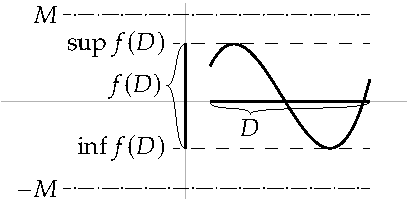
\includegraphics{figures/boundedfunc}
\caption{Example of a bounded function, a bound $M$, and its supremum and infimum.\label{boundedfuncfig}}
\end{myfigureht}
For a function $f \colon D \to \R$, we write
(see \figureref{boundedfuncfig} for
an example)
\glsadd{not:supf}\glsadd{not:inff}
\begin{align*}
& \sup_{x \in D} f(x) := \sup\, f(D) , \\
& \inf_{x \in D} f(x) := \inf\, f(D) .
\end{align*}
We also sometimes replace the \myquote{$x \in D$} with an expression.
For example if, as before, $f(x) = x^2-9x+1$, for $-1 \leq x \leq 5$, 
a little bit of calculus shows
\begin{equation*}
\sup_{x \in D} f(x) = 
\sup_{-1 \leq x \leq 5} ( x^2 -9x+1 ) = 11,
\qquad
\inf_{x \in D} f(x) = 
\inf_{-1 \leq x \leq 5} ( x^2 -9x+1 ) = \nicefrac{-77}{4} .
\end{equation*}



\begin{prop} \label{prop:funcsupinf}
If $f \colon D \to \R$ and $g \colon D \to \R$ ($D$ nonempty) are
bounded\footnote{The boundedness hypothesis is for simplicity,
it can be dropped if we allow for the extended real numbers.}
functions and
\begin{equation*}
f(x) \leq g(x) \qquad \text{for all } x \in D,
\end{equation*}
then
\begin{equation} \label{prop:funcsupinf:eq}
\sup_{x \in D} f(x) \leq \sup_{x \in D} g(x)
\qquad \text{and} \qquad
\inf_{x \in D} f(x) \leq \inf_{x \in D} g(x) .
\end{equation}
\end{prop}

Be careful with the variables.  The $x$ on the left side of
the inequality in \eqref{prop:funcsupinf:eq}
is different from the $x$ on the right.  You
should really think of, say, the first inequality as
\begin{equation*}
\sup_{x \in D} f(x) \leq \sup_{y \in D} g(y) .
\end{equation*}
Let us prove this inequality.  If $b$ is an upper bound for $g(D)$, then
$f(x) \leq g(x) \leq b$ for all $x \in D$, and hence $b$ is also an upper
bound for $f(D)$,
or $f(x) \leq b$ for all $x \in D$.
Take the least upper bound of $g(D)$ to get that for all $x \in D$
\begin{equation*}
f(x) \leq \sup_{y \in D} g(y) .
\end{equation*}
Therefore,
$\sup_{y \in D} g(y)$ is an upper bound for $f(D)$ and thus greater than or
equal to the least upper bound of $f(D)$.
\begin{equation*}
\sup_{x \in D} f(x) \leq \sup_{y \in D} g(y) .
\end{equation*}
The second inequality (the statement about the inf) is left as an exercise
(\exerciseref{exercise:finishfuncsupinf}).

\medskip

A common mistake is to conclude 
\begin{equation} \label{rn:av:ltnottrue}
\sup_{x \in D} f(x) \leq \inf_{y \in D} g(y) .
\end{equation}
The inequality \eqref{rn:av:ltnottrue} is not true given the hypothesis of
the proposition above.  For this stronger
inequality we need the stronger hypothesis
\begin{equation*}
f(x) \leq g(y) \qquad \text{for all } x \in D \text{ and } y \in D.
\end{equation*}
The proof as well as a counterexample is left as an exercise
(\exerciseref{exercise:supinffuncineq}).

\subsection{Exercises}

\begin{exercise}
Show that
$\abs{x-y} < \epsilon$ if and only if $x-\epsilon < y < x+\epsilon$.
\end{exercise}

\begin{exercise}
Show: \qquad
%\begin{enumerate}[a)]
%\item
a)
$\max \{x,y\} = \frac{x+y+\abs{x-y}}{2}$
%\item
\qquad
b)
$\min \{x,y\} = \frac{x+y-\abs{x-y}}{2}$
%\end{enumerate}
\end{exercise}

\begin{exercise}
Find a number $M$ such that $\sabs{x^3-x^2+8x} \leq M$ for all $-2 \leq x \leq
10$.
\end{exercise}

\begin{exercise} \label{exercise:finishfuncsupinf}
Finish the proof of \propref{prop:funcsupinf}.
That is, prove that
given a set $D$,
and two bounded functions
$f \colon D \to \R$ and $g \colon D \to \R$ 
such that $f(x) \leq g(x)$ for all $x \in D$, then 
\begin{equation*}
\inf_{x\in D} f(x) \leq \inf_{x\in D} g(x) .
\end{equation*}
\end{exercise}

\begin{exercise} \label{exercise:supinffuncineq}
Let 
$f \colon D \to \R$ and $g \colon D \to \R$ be functions ($D$ nonempty).
\begin{enumerate}[a)]
%
\item
Suppose 
$f(x) \leq g(y)$ for all $x \in D$ and $y \in D$.  Show that
\begin{equation*}
\sup_{x\in D} f(x) \leq \inf_{x\in D} g(x) .
\end{equation*}
%
\item
Find a specific $D$, $f$, and $g$, such that
$f(x) \leq g(x)$ for all $x \in D$, but
\begin{equation*}
\sup_{x\in D} f(x) > \inf_{x\in D} g(x) .
\end{equation*}
\end{enumerate}
\end{exercise}

\begin{exercise}
Prove \propref{prop:funcsupinf} without the assumption that
the functions are bounded.  Hint: You need to use the extended real
numbers.
\end{exercise}

\begin{exercise} \label{exercise:sumofsup}
Let $D$ be a nonempty set.
Suppose $f \colon D \to \R$ and $g \colon D \to \R$ are bounded functions.
\begin{enumerate}[a)]
\item
Show 
\begin{equation*}
\sup_{x\in D} \bigl(f(x) + g(x) \bigr) \leq
\sup_{x\in D} f(x)
+
\sup_{x\in D} g(x)
\qquad \text{and} \qquad
\inf_{x\in D} \bigl(f(x) + g(x) \bigr) \geq
\inf_{x\in D} f(x)
+
\inf_{x\in D} g(x) .
\end{equation*}
\item
Find examples where we obtain strict inequalities.
\end{enumerate}
\end{exercise}

\begin{exercise}
Suppose $f \colon D \to \R$ and $g \colon D \to \R$ are bounded functions
and
$\alpha \in \R$.
\begin{enumerate}[a)]
\item
Show that $\alpha f \colon D \to \R$ defined by $(\alpha f) (x) := \alpha
f(x)$ is a bounded function.
\item
Show that $f+g \colon D \to \R$ defined by $(f+g) (x) := f(x) + g(x)$
is a bounded function.
\end{enumerate}
\end{exercise}

\begin{exercise}
Let $f \colon D \to \R$ and $g \colon D \to \R$ be functions, $\alpha \in
\R$, and
recall what $f+g$ and $\alpha f$ means from the previous exercise.
\begin{enumerate}[a)]
\item
Prove that if $f+g$ and $g$ are bounded, then $f$ is bounded.
\item
Find an example where $f$ and $g$ are both unbounded, but $f+g$ is
bounded.
\item
Prove that if $f$ is bounded but $g$ is unbounded, then $f+g$ is
unbounded.
\item
Find an example where $f$ is unbounded but $\alpha f$ is bounded.
\end{enumerate}
\end{exercise}

%%%%%%%%%%%%%%%%%%%%%%%%%%%%%%%%%%%%%%%%%%%%%%%%%%%%%%%%%%%%%%%%%%%%%%%%%%%%%%

\sectionnewpage
\section{Intervals and the size of \texorpdfstring{$\R$}{R}}
\label{sec:intandsizeR}

\sectionnotes{0.5--1 lecture (proof of uncountability of $\R$ can be optional)}

You surely saw the notation for intervals\index{interval}
before, but let us give a formal
definition here.  For $a,  b \in \R$ such that $a < b$, we define
\glsadd{not:openbdinterval}%
\glsadd{not:closedbdinterval}%
\glsadd{not:halfopenbdinterval}%
\glsadd{not:openubdinterval}%
\glsadd{not:closedubdinterval}%
\begin{align*}
& [a,b] := \{ x \in \R : a \leq x \leq b \}, \\
& (a,b) := \{ x \in \R : a < x < b \}, \\
& (a,b] := \{ x \in \R : a < x \leq b \}, \\
& [a,b) := \{ x \in \R : a \leq x < b \} .
\end{align*}
The interval $[a,b]$ is called a \emph{\myindex{closed interval}}
and $(a,b)$ is called an \emph{\myindex{open interval}}.  The intervals
of the form $(a,b]$ and $[a,b)$ are called
\emph{half-open intervals}\index{half-open interval}.

The intervals above are \emph{bounded intervals}\index{bounded
interval}, since both $a$ and $b$ are real numbers.  We 
define \emph{unbounded intervals}\index{unbounded interval},
\begin{align*}
& [a,\infty) := \{ x \in \R : a \leq x \}, \\
& (a,\infty) := \{ x \in \R : a < x \}, \\
& (-\infty,b] := \{ x \in \R : x \leq b \}, \\
& (-\infty,b) := \{ x \in \R : x < b \} .
\end{align*}
For completeness, we define $(-\infty,\infty) := \R$.
The intervals $[a,\infty)$, $(-\infty,b]$, and $\R$ are sometimes called
\emph{\myindex{unbounded closed intervals}},
and $(a,\infty)$, $(-\infty,b)$, and $\R$ are sometimes called
\emph{\myindex{unbounded open intervals}}.

The proof of the following proposition is left as an exercise.
In short, an interval is a set with at least two points
that contains all points between any two
points.\footnote{Sometimes single point sets and the empty set are
also called intervals, but in this book, intervals have at least 2 points.
That is, we only defined the bounded intervals if $a < b$.}

\begin{prop} \label{prop:intervaldef}
A set $I \subset \R$ is an interval if and only if
$I$ contains at least 2 points and
for all $a,c \in I$ and $b \in \R$ such that $a < b < c$, we have $b \in I$.
\end{prop}

We have already seen that every open interval $(a,b)$ (where $a < b$ of course)
must be nonempty.  For example, it contains the number $\frac{a+b}{2}$.
An unexpected fact is that from a set-theoretic perspective,
all intervals have the same \myquote{size,} that is, they all have
the same cardinality.  For example the map $f(x) := 2x$
takes the interval $[0,1]$ bijectively to the interval $[0,2]$.

Maybe more interestingly,
the function $f(x) := \tan(x)$
is a bijective map from $(-\nicefrac{\pi}{2},\nicefrac{\pi}{2})$ to $\R$.  Hence the bounded
interval $(-\nicefrac{\pi}{2},\nicefrac{\pi}{2})$ has the same cardinality as $\R$.  It is not
completely straightforward to construct a bijective map from $[0,1]$ to
$(0,1)$, but it is possible.

And do not worry, there does exist a way to measure the \myquote{size} of subsets
of real numbers that
\myquote{sees}
the difference between $[0,1]$ and $[0,2]$.  However, its proper definition
requires much more machinery than we have right now.

Let us say more about the cardinality of intervals and hence about the
cardinality of $\R$.  We have seen that there exist irrational numbers, that is
$\R \setminus \Q$, is nonempty.  The question is: How many irrational numbers
are there?  It turns out there are a lot more irrational numbers than rational
numbers.  We have seen that $\Q$ is countable, and we will show 
that $\R$ is uncountable.
In fact, the cardinality of $\R$ is the
same as the cardinality of $\sP(\N)$, although we will not prove this
claim here.

\begin{thm}[Cantor]\index{Cantor's theorem}
$\R$ is uncountable.
\end{thm}

We give a version of
Cantor's original proof from
1874 as this proof requires the least setup.  Normally this proof is stated
as a contradiction, but a proof by contrapositive is easier to
understand.

\begin{proof}
Let $X \subset \R$ be a countably infinite
subset such that for every pair of real numbers
$a < b$, there is an $x \in X$ such that $a < x < b$.  Were $\R$ countable,
we could take $X = \R$.  We will show that $X$ is necessarily
a proper subset, and so $X$ cannot equal $\R$, and $\R$ must be
uncountable.

As $X$ is countably infinite, 
there is a bijection from $\N$ to $X$.  We write $X$ as
a sequence of real numbers $x_1, x_2, x_3,\ldots$, such that
each number in $X$
is given by $x_n$ for some $n \in \N$.

We inductively
construct two sequences of real numbers $a_1,a_2,a_3,\ldots$ and
$b_1,b_2,b_3,\ldots$.  Let
$a_1 := x_1$ and $b_1 := x_1+1$.
Note that $a_1 < b_1$ and
$x_1 \notin (a_1,b_1)$.
For some $k > 1$,
suppose $a_1,a_2,\ldots,a_{k-1}$ and $b_1,b_2,\ldots,b_{k-1}$ have been
defined,
suppose
$a_1 < a_2 < \cdots < a_{k-1} < b_{k-1} < \cdots < b_2 < b_1$,
and suppose
for each $j=1,2,\ldots,k-1$,
we have $x_\ell \notin (a_{j},b_{j})$ 
for $\ell=1,2,\ldots,j$.
\begin{enumerate}[(i)]
\item Define $a_k := x_n$, where $n$ is the smallest $n \in \N$
such that $x_n \in (a_{k-1},b_{k-1})$.  Such an $x_n$ exists by our
assumption on $X$, and $n \geq k$ by the assumption on $(a_{k-1},b_{k-1})$.
\item Next, define $b_k$ to be some real number in $(a_{k},b_{k-1})$.
\end{enumerate}
Notice that %$a_k < b_k$ and
$a_{k-1} < a_k < b_k < b_{k-1}$.
Also notice that $(a_{k},b_{k})$ does not contain $x_k$ and hence
does not contain $x_j$ for $j=1,2,\ldots,k$.
The two sequences are now defined.

Claim: \emph{$a_n < b_m$ for all $n$ and $m$ in $\N$.} Proof: Let us first
assume $n < m$.  Then $a_n < a_{n+1} < \cdots < a_{m-1} < a_m < b_m$.
Similarly for $n > m$.  The claim follows.

Let $A := \{ a_n : n \in \N \}$ and $B := \{ b_n : n \in \N \}$.
By \propref{infsupineq:prop} and the claim above,
\begin{equation*}
\sup\, A \leq \inf\, B .
\end{equation*}
Define $y := \sup\, A$.  The number $y$ cannot be a member of $A$:  If $y = a_n$
for some $n$, then $y < a_{n+1}$, which is impossible.
Similarly, $y$ cannot be a member of $B$.  Therefore,
$a_n < y$ for all $n\in \N$
and $y < b_n$ for all $n\in \N$.
In other words, for every $n \in \N$, we have $y \in (a_n,b_n)$.
By the construction of the sequence, $x_n \not\in (a_n,b_n)$,
and so $y \not= x_n$.  As this was true for all $n \in \N$, we have that $y
\not\in X$.

We have constructed a real number $y$ that is not in $X$, and thus $X$
is a proper subset of $\R$.
The sequence $x_1,x_2,\ldots$ cannot contain all elements of $\R$
and thus $\R$ is uncountable.
\end{proof}

\subsection{Exercises}

\begin{exercise}
For $a < b$, construct an explicit bijection from $(a,b]$ to $(0,1]$.
\end{exercise}

\begin{exercise}
Suppose $f \colon [0,1] \to (0,1)$ is a bijection.
Using $f$, construct a
bijection from $[-1,1]$ to $\R$.
\end{exercise}

\begin{exercise} \label{exercise:intervaldef}
Prove \propref{prop:intervaldef}.
That is,
suppose $I \subset \R$ is a subset with at least 2 elements
such that if $a < b < c$ and $a, c \in I$, then $b \in I$.
Prove that $I$ is one of the nine types of intervals explicitly
given in this section.
Furthermore, prove that the intervals given in this section
all satisfy this property.
\end{exercise}

\begin{exercise}[Hard]
Construct an explicit bijection from $(0,1]$ to $(0,1)$.
Hint: One approach is as follows: First map $(\nicefrac{1}{2},1]$
to $(0,\nicefrac{1}{2}]$, then map
$(\nicefrac{1}{4},\nicefrac{1}{2}]$
to $(\nicefrac{1}{2},\nicefrac{3}{4}]$, etc.
Write down the map explicitly, that
is, write down an algorithm that tells you exactly what number goes where.
Then prove that the map is a bijection.
\end{exercise}

\begin{exercise}[Hard]
Construct an explicit bijection from $[0,1]$ to $(0,1)$.
\end{exercise}

\begin{exercise}
\leavevmode
\begin{enumerate}[a)]
\item
Show that every closed interval $[a,b]$ is the intersection
of countably many open intervals.
\item
Show that every open interval $(a,b)$
is a countable union of closed intervals.
\item
Show that an intersection
of a possibly infinite family of bounded closed intervals,
$\bigcap\limits_{\lambda \in I} [a_\lambda,b_\lambda]$,
is either empty, a single point,
or a bounded closed interval.
\end{enumerate}
\end{exercise}

\begin{exercise}
Suppose $S$ is a set of disjoint open intervals in $\R$.  That is, 
if $(a,b) \in S$ and $(c,d) \in S$, then either $(a,b) = (c,d)$
or $(a,b) \cap (c,d) = \emptyset$.  Prove $S$ is a countable set.
\end{exercise}

\begin{exercise}
Prove that the cardinality of $[0,1]$ is the same as the cardinality of
$(0,1)$ by showing that
$\abs{[0,1]} \leq \abs{(0,1)}$ and
$\abs{(0,1)} \leq \abs{[0,1]}$.  See 
\defnref{def:comparecards}.
This proof requires the Cantor--Bernstein--Schr\"oder theorem we
stated without proof.  Note that this proof does not give you an
explicit bijection.
\end{exercise}

\begin{exercise}[Challenging]
A number $x$ is \emph{algebraic}\index{algebraic number} if $x$ is a root of a polynomial with
integer coefficients, in other words, $a_n x^n + a_{n-1} x^{n-1}  + \cdots
+ a_1 x + a_0 = 0$ where $a_0,a_1,\ldots,a_n \in \Z$.
\begin{enumerate}[a)]
\item
Show that there are only
countably many algebraic numbers.
\item
Show that there exist non-algebraic (transcendental)
numbers (follow in the footsteps of Cantor, use the uncountability of $\R$).
\end{enumerate}
Hint: Feel free to use the fact that a polynomial of degree $n$ has at most $n$ real
roots.
\end{exercise}

\begin{exercise}[Challenging]
Let $F$ be the set of all functions $f \colon \R \to \R$.
Prove $\abs{\R} < \abs{F}$
using Cantor's \thmref{cantorspowersetthm}.\footnote{Interestingly,
if $C$ is the set of continuous functions, then $\abs{\R} = \abs{C}$.}
\end{exercise}

%%%%%%%%%%%%%%%%%%%%%%%%%%%%%%%%%%%%%%%%%%%%%%%%%%%%%%%%%%%%%%%%%%%%%%%%%%%%%%

\sectionnewpage
\section{Decimal representation of the reals}
\label{sec:decimals}

\sectionnotes{1 lecture (optional)}

We often think of real numbers as their
\emph{\myindex{decimal representation}}.  For
a positive integer $n$, we find the digits $d_K,d_{K-1},\ldots,d_2,d_1,d_0$ for some
$K$,
where each $d_j$ is an integer between $0$ and $9$, then
\begin{equation*}
n = d_K {10}^K + d_{K-1} {10}^{K-1} + \cdots + d_2 {10}^2 + d_1 10 + d_0 .
\end{equation*}
We often assume $d_K \not= 0$.  To represent $n$ we write the sequence of
digits: $n = d_K d_{K-1} \cdots d_2 d_1 d_0$.
By a (decimal)
\emph{\myindex{digit}}\index{decimal digit}, we mean an integer
between $0$ and $9$.

Similarly, we
represent some rational numbers.  That is, for certain
numbers $x$, we can find
negative integer $-M$, a positive integer $K$, and digits
$d_K,d_{K-1},\ldots,d_1,d_0,d_{-1},\ldots,d_{-M}$, such that
\begin{equation*}
x = d_K {10}^K + d_{K-1} {10}^{K-1} + \cdots + d_2 {10}^2 + d_1 10 + d_0 
+ d_{-1} {10}^{-1} + d_{-2} {10}^{-2} + \cdots + d_{-M} {10}^{-M} .
\end{equation*}
We write $x = d_K d_{K-1} \cdots d_1 d_0 \, . \, d_{-1} d_{-2} \cdots d_{-M}$.

Not every real number has such a representation, even the simple
rational number $\nicefrac{1}{3}$ does not.  The irrational number $\sqrt{2}$ 
does not have such a representation either.  To get a representation for
all real numbers, we must allow infinitely many digits.

Let us consider only real numbers in the interval $(0,1]$.  If
we find a representation for these, adding 
integers to them obtains a representation for all real numbers.
Take an infinite sequence of decimal digits:
\begin{equation*}
0.d_1d_2d_3\ldots.
\end{equation*}
That is, we have a digit $d_j$ for every $j \in \N$.
We renumbered the digits to avoid the negative signs.
We call the number
\begin{equation*}
D_n := 
\frac{d_1}{10} + 
\frac{d_2}{{10}^2} + 
\frac{d_3}{{10}^3} + 
\cdots +
\frac{d_n}{{10}^n} .
\end{equation*}
the truncation of $x$ to $n$ decimal digits.
We say this
sequence of digits represents a real number $x$ if
\begin{equation*}
x =
\sup_{n \in \N} \left(
\frac{d_1}{10} + 
\frac{d_2}{{10}^2} + 
\frac{d_3}{{10}^3} + 
\cdots +
\frac{d_n}{{10}^n}
\right) =
\sup_{n \in \N} \, D_n .
\end{equation*}

\begin{prop} \label{prop:decimalprop}
\leavevmode
\begin{enumerate}[(i)]
\item
Every infinite sequence of digits
$0.d_1d_2d_3\ldots$ represents a unique real number $x \in [0,1]$, and
\begin{equation*}
D_n \leq x \leq D_n+\frac{1}{{10}^n} \qquad \text{for all } n \in \N.
\end{equation*}
\item
For every $x \in (0,1]$ there exists an infinite sequence of digits
$0.d_1d_2d_3\ldots$ that represents $x$.
There exists a unique representation such that
\begin{equation*}
D_n < x \leq D_n+\frac{1}{{10}^n} \qquad \text{for all } n \in \N.
\end{equation*}
\end{enumerate}
\end{prop}

\begin{proof}
We start with the first item.  Take an arbitrary infinite sequence of
digits $0.d_1d_2d_3\ldots$.  Use the geometric sum formula to write
\begin{equation*}
\begin{split}
D_n =
\frac{d_1}{10} + 
\frac{d_2}{{10}^2} + 
\frac{d_3}{{10}^3} + 
\cdots +
\frac{d_n}{{10}^n} 
& \leq
\frac{9}{10} + 
\frac{9}{{10}^2} + 
\frac{9}{{10}^3} + 
\cdots +
\frac{9}{{10}^n} 
\\
& =
\frac{9}{10}
\bigl( 1 + \nicefrac{1}{10} + 
{(\nicefrac{1}{10})}^2 + \cdots + 
{(\nicefrac{1}{10})}^{n-1} \bigr)
\\
& =
\frac{9}{10}
\left(
\frac{1-{(\nicefrac{1}{10})}^{n}}{1-\nicefrac{1}{10}}
\right)
= 1-{(\nicefrac{1}{10})}^{n}
< 1 .
\end{split}
\end{equation*}
In particular, $D_n < 1$ for all $n$.  A sum of nonnegative numbers is
nonnegative so $D_n \geq 0$, and hence
\begin{equation*}
0 \leq \sup_{n\in \N} \, D_n \leq 1 .
\end{equation*}
Therefore, $0.d_1d_2d_3\ldots$ represents a unique number $x := \sup_{n\in
\N} D_n \in [0,1]$.
As $x$ is a supremum, then $D_n \leq x$.
Take $m \in \N$.  If $m < n$, then $D_m - D_n \leq 0$.  If $m > n$, then
computing as above
\begin{equation*}
D_m - D_n
=
\frac{d_{n+1}}{{10}^{n+1}} + 
\frac{d_{n+2}}{{10}^{n+2}} + 
\frac{d_{n+3}}{{10}^{n+3}} + 
\cdots +
\frac{d_{m}}{{10}^m} 
\leq
\frac{1}{{10}^{n}}
\bigl(
1-{(\nicefrac{1}{10})}^{m-n}
\bigr)
<
\frac{1}{{10}^{n}} .
\end{equation*}
Take the supremum over $m$ to find
\begin{equation*}
x - D_n
\leq
\frac{1}{{10}^{n}} .
\end{equation*}

We move on to the
second item.  Take any $x \in (0,1]$.
First let us tackle the existence.
For convenience, let $D_0 := 0$.
Then,
$D_0 < x \leq D_0 + {10}^{-0}$.
Suppose we defined the digits $d_1,d_2,\ldots,d_n$,
and that 
$D_k < x \leq D_k + {10}^{-k}$, for $k=0,1,2,\ldots,n$.  We need to define $d_{n+1}$.

By the 
\hyperref[thm:arch:i]{Archimedean property} of the real numbers,
find an integer $j$ such that
$x-D_n \leq j {10}^{-(n+1)}$.  Take the least such $j$ and obtain 
\begin{equation} \label{eq:theDnjineq}
(j-1){10}^{-(n+1)} < x-D_n \leq j {10}^{-(n+1)} .
\end{equation}
Let $d_{n+1} := j-1$.
As $D_n < x$,
then $d_{n+1} = j-1 \geq 0$.  On the other hand, since
$x-D_n \leq {10}^{-n}$, we have that
$j$ is at most 10, and therefore $d_{n+1} \leq 9$.
So $d_{n+1}$ is a
decimal digit.
Since $D_{n+1} = D_n + d_{n+1} {10}^{-(n+1)}$
add $D_n$ to the inequality
\eqref{eq:theDnjineq} above:
\begin{multline*}
D_{n+1} = D_n + (j-1){10}^{-(n+1)} < x
\leq
D_n + j {10}^{-(n+1)} \\
=
D_n + (j-1) {10}^{-(n+1)} +
{10}^{-(n+1)} = D_{n+1} + {10}^{-(n+1)} .
\end{multline*}
And so
$D_{n+1} < x \leq D_{n+1} + {10}^{-(n+1)}$ holds.
We inductively
defined an infinite sequence of digits $0.d_1d_2d_3\ldots$.

Consider $D_{n} < x \leq D_{n} + {10}^{-n}$.
As $D_n < x$ for all $n$, then
$\sup \{ D_n : n \in \N \} \leq x$.
The second inequality for $D_n$ implies
\begin{equation*}
x - \sup \{ D_m : m \in \N \}
\leq
x - D_n \leq 10^{-n} .
\end{equation*}
As the inequality holds for all $n$ and
${10}^{-n}$ can be made arbitrarily small (see
\exerciseref{exercise:bnlimit}), we have $x \leq 
\sup \{ D_m : m \in \N \}$.
Therefore,
$\sup \{ D_m : m \in \N \} = x$.

What is left to show is the uniqueness.
Suppose $0.e_1e_2e_3\ldots$ is another representation of $x$.
Let $E_n$ be the $n$-digit truncation of $0.e_1e_2e_3\ldots$, and suppose
$E_n < x \leq E_n + {10}^{-n}$ for all $n \in \N$.
Suppose for some $K \in \N$, $e_n = d_n$ for all $n < K$, so
$D_{K-1} = E_{K-1}$.  Then
\begin{equation*}
E_K = D_{K-1} + e_K{10}^{-K} < x \leq E_K + {10}^{-K} = D_{K-1} +
e_K{10}^{-K} + {10}^{-K} .
\end{equation*}
Subtracting $D_{K-1}$ and multiplying by ${10}^{K}$ we get
\begin{equation*}
e_K < (x - D_{K-1}){10}^K \leq e_K + 1 .
\end{equation*}
Similarly,
\begin{equation*}
d_K < (x - D_{K-1}){10}^K \leq d_K + 1 .
\end{equation*}
Hence, both $e_K$ and $d_K$ are the largest integer $j$
such that $j < (x - D_{K-1}){10}^K$, and therefore $e_K = d_K$.  That is,
the representation is unique.
\end{proof}

The representation is not unique if we do not require
$D_n < x$ for all $n$.
For example, for the
number $\nicefrac{1}{2}$, the method in the proof obtains the representation
\begin{equation*}
0.49999\ldots .
\end{equation*}
However, $\nicefrac{1}{2}$ also has the representation $0.50000\ldots$.

The only numbers that have nonunique
representations are ones that end either in an infinite sequence of $0$s
or $9$s, because the only representation for which
$D_n = x$ is one where all digits past the $n$th digit are zero.  In this case
there are exactly two representations of $x$ (see the exercises).

Let us give another proof of the uncountability of the reals using decimal
representations.
This is Cantor's second proof, and is probably better known.
This proof may seem shorter, but it is because we already did
the hard part above and we are left with a slick trick to prove that $\R$ is
uncountable.  This trick is called
\emph{\myindex{Cantor diagonalization}}\index{diagonalization} and
finds use in other proofs as well.

\begin{thm}[Cantor]
The set $(0,1]$ is uncountable.
\end{thm}

\begin{proof}
Let $X := \{ x_1,x_2,x_3,\ldots \}$ be any countable subset of real numbers in $(0,1]$.
We will construct a real number not in $X$.  Let
\begin{equation*}
x_n = 0.d_1^nd_2^nd_3^n\ldots
\end{equation*}
be the unique representation from the proposition, that is, $d_j^n$ is the
$j$th digit of the $n$th number.  Let
\begin{equation*}
e_n :=
\begin{cases}
1 & \text{if } d_n^n \not= 1, \\
2 & \text{if } d_n^n = 1.
\end{cases}
\end{equation*}
Let $E_n$ be the $n$-digit truncation of $y = 0.e_1e_2e_3\ldots$.  Because
all the digits are nonzero we get $E_n < E_{n+1} \leq y$.  Therefore
\begin{equation*}
E_n < y \leq E_n + {10}^{-n} 
\end{equation*}
for all $n$, and the representation is the unique one for $y$ from 
the proposition.  For every $n$, the $n$th digit
of $y$ is different from the $n$th digit of $x_n$, so $y \not= x_n$.
Therefore $y \notin X$, and as $X$ was an arbitrary countable subset,
$(0,1]$ must be uncountable.  See \figureref{cantorexamplefig} for an
example.
\begin{myfigureht}
\subimport*{figures/}{cantorexamplefig.pdf_t}
\caption{Example of Cantor diagonalization, the diagonal digits $d_n^n$
marked.\label{cantorexamplefig}}
\end{myfigureht}
\end{proof}

Using decimal digits we can also find lots of numbers that are not rational.
The following proposition is true for every
rational number, but we give it only for $x \in (0,1]$ for simplicity.

\begin{prop} \label{prop:rationaldecimal}
If $x \in (0,1]$ is a rational number and $x = 0.d_1d_2d_3\ldots$,
then the decimal digits eventually start repeating.  That is, there are 
positive integers $N$ and $P$, such that for all $n \geq N$, $d_n = d_{n+P}$.
\end{prop}

\begin{proof}
Suppose $x = \nicefrac{p}{q}$ for positive integers $p$ and $q$.
Suppose also that $x$ is a number with a unique representation, as
otherwise we have seen above that both its representations are repeating,
see also \exerciseref{exercise:nonuniquedecimals}.  This also means
that $x \not= 1$ so $p < q$.

To compute the first digit we take $10 p$ and divide by
$q$.  Let $d_1$ be the quotient, and the remainder $r_1$ is some integer
between 0 and $q-1$.  That is, $d_1$ is the largest integer
such that $d_1 q \leq 10p$ and then $r_1 = 10p - d_1q$.
As $p < q$, then $d_1 < 10$, so $d_1$ is a digit.
Furthermore,
\begin{equation*}
\frac{d_1}{10} \leq \frac{p}{q} =
\frac{d_1}{10} + \frac{r_1}{10q} \leq \frac{d_1}{10} +
\frac{1}{10} .
\end{equation*}
The first inequality must be strict since $x$ has a
unique representation.  That is, $d_1$ really is the first digit.
What is left is $\nicefrac{r_1}{(10q)}$.  This is the same as computing the
first digit of $\nicefrac{r_1}{q}$.
To compute $d_2$ divide $10 r_1$ by $q$, and so on.
After computing $n-1$ digits, we have
$\nicefrac{p}{q} = D_{n-1} + \nicefrac{r_{n-1}}{(10^{n} q)}$.
To get the $n$th digit,
divide $10 r_{n-1}$ by $q$
to get quotient $d_n$, remainder $r_n$, and the inequalities
\begin{equation*}
\frac{d_n}{10} \leq \frac{r_{n-1}}{q} =
\frac{d_n}{10} + \frac{r_n}{10q} \leq \frac{d_n}{10} +
\frac{1}{10} .
\end{equation*}
Dividing by $10^{n-1}$ and adding $D_{n-1}$ we find
\begin{equation*}
D_n \leq D_{n-1} + \frac{r_{n-1}}{10^{n} q} = \frac{p}{q} \leq D_n +
\frac{1}{10^n} .
\end{equation*}
By uniqueness we really have 
the $n$th digit $d_n$ from the construction.

The new digit depends only the remainder from the previous
step.  There
are at most $q$ possible remainders
and hence at some step the process must start repeating itself,
and $P$ is at most $q$.
\end{proof}

The converse of the proposition is also true and is left as an exercise.

\begin{example}
The number
\begin{equation*}
x = 0.101001000100001000001\ldots,
\end{equation*}
is irrational.
That is, the digits are $n$ zeros, then a one, then $n+1$
zeros, then a one, and so on and so forth.
The fact that $x$ is irrational follows from the
proposition; the digits never start repeating.
For every $P$,
if we go far enough, we find a 1 followed by at least $P+1$ zeros.
\end{example}

\subsection{Exercises}

\begin{exercise}[Easy]
What is the decimal representation of $1$ guaranteed by
\propref{prop:decimalprop}?  Make sure to show that it does satisfy
the condition.
\end{exercise}

\begin{exercise}
Prove the converse of \propref{prop:rationaldecimal}, that is,
if the digits in the decimal representation of $x$ are eventually repeating, then 
$x$ must be rational.
\end{exercise}

\begin{exercise} \label{exercise:nonuniquedecimals}
Show that real numbers $x \in (0,1)$ with nonunique decimal representation
are exactly the rational numbers that can be written
as $\frac{m}{10^n}$ for some integers $m$ and $n$.  In this case show that
there exist exactly two representations of $x$.
\end{exercise}

\begin{exercise} \label{exercise:decimalpropbaseb}
Let $b \geq 2$ be an integer.  Define a representation of a real number in
$[0,1]$ in terms of base $b$ rather than base 10 and prove
\propref{prop:decimalprop} for base $b$.
\end{exercise}

\begin{exercise}
Using the previous exercise with $b=2$ (binary), 
show that cardinality of $\R$ is the same as the cardinality of $\sP(\N)$,
obtaining yet another (though related) proof that $\R$ is uncountable.
Hint: Construct two injections, one from $[0,1]$ to $\sP(\N)$
and one from $\sP(\N)$ to $[0,1]$.  Hint 2: Given a
set $A \subset \N$, let the $n$th binary digit of $x$ be 1 if $n\in A$.
\end{exercise}

\begin{exercise}[Challenging]
Explicitly construct an injection from $[0,1] \times [0,1]$ to $[0,1]$ (think about why
this is so surprising\footnote{%
With quite a bit more work (or by applying the
Cantor--Bernstein--Schr\"oder theorem)
one can prove that there is a bijection.
When he proved this result, Cantor apparently wrote
\myquote{I see it but I don't believe it.}}).
Then describe the set of numbers in $[0,1]$ not in the image of your
injection (unless, of course, you managed to construct a bijection).
Hint: Consider even and odd digits of the decimal expansion.
\end{exercise}

\begin{exercise}
Prove that if $x = \nicefrac{p}{q} \in (0,1]$ is a rational number, $q > 1$,
then the period $P$ of repeating digits in the decimal representation
of $x$ is in fact less than or equal to $q-1$.
\end{exercise}

\begin{exercise} \label{exercise:bnlimit}
Prove that if $b \in \N$ and $b \geq 2$, then for every $\epsilon > 0$,
there is an $n \in \N$ such that 
$b^{-n} < \epsilon$.  Hint:
One possibility is to first prove that $b^n > n$ for all $n \in \N$ by induction.
\end{exercise}

\begin{exercise}
Explicitly construct an injection $f \colon \R \to \R \setminus \Q$ using
\propref{prop:rationaldecimal}.
\end{exercise}
